\documentclass[11pt,a4paper]{article}
\usepackage[margin=2.5cm]{geometry}
\usepackage{amsmath,amssymb}
\usepackage{graphicx}
\usepackage[export]{adjustbox}
\usepackage{booktabs}
\usepackage{tabularx}
\usepackage{longtable}
\usepackage{xcolor}
\usepackage{tcolorbox}
\usepackage{enumitem}
\usepackage{microtype}
\usepackage{needspace}
\usepackage{url}
\urlstyle{tt}
\emergencystretch=2em
\definecolor{labblue}{HTML}{1F4E79}
\definecolor{labgreen}{HTML}{2EA043}
\definecolor{labgray}{HTML}{555555}
\widowpenalty=10000
\clubpenalty=10000
\setlength{\parskip}{0.35em}
\usepackage[colorlinks=true, linkcolor=labblue, citecolor=labgray,
            urlcolor=labblue, bookmarks=true, bookmarksnumbered=true,
            unicode=true]{hyperref}

\hypersetup{
    pdftitle={Zitterbewegung at $\omega = 2E$: Trembling Motion from Interband Coherence},
    pdfauthor={Isaev, Iskhak Khamzatovich},
    pdfsubject={AB-Cloud Dirac Laboratory — per-test monograph D6},
    pdfkeywords={Dirac equation, Hofstadter model, Riemann zeta zeros, AB-Cloud, D6}
}
\begin{document}

\noindent{\small\color{labgray}\texttt{AB-Cloud Dirac Laboratory · per-test monograph · D6 · seed 96 · v1.4}}\\[0.3em]
\rule{\textwidth}{0.8pt}\\[0.6em]
{\LARGE\bfseries\color{labblue} Zitterbewegung at $\omega = 2E$: Trembling Motion from Interband Coherence}\\[0.5em]
{\normalsize\itshape Test D6 — frequency ratios $0.99958$ (box) and $0.9998$ (torus dipole)}\\[0.4em]
\rule{\textwidth}{0.4pt}

\begin{tcolorbox}[colback=labgreen!8, colframe=labgreen!70!black, title={Verdict: PASS — 2/2 checks}, fonttitle=\bfseries, boxrule=0.6pt]
\textbf{Abstract.} Test D6 verifies Zitterbewegung -- the trembling motion of a Dirac particle caused by interference between positive- and negative-energy components -- with two independent instruments: a 1D Dirac box where the trembling frequency ratio $\omega/2E = 0.999583$ is measured from the position oscillation, and the laboratory torus where the interband dipole oscillates at $\omega/2E_1 = 0.9998$ \cite{schrodinger,dirac}. A sublattice-mixing control kills the oscillation in both setups, confirming that the mechanism is interband coherence and nothing else. The test closes the clean-suite programme: kinematics (D1), structure (D2), geometry (D3), magnetics (D4) and now real-time dynamics (D5, D6) all read Dirac.
\end{tcolorbox}

\section{What This Test Verifies}
Zitterbewegung was identified by Schrödinger in 1930: a Dirac wave packet built from both energy bands has an expectation value of position that trembles at frequency $\omega = 2E$ -- the beat between the positive- and negative-energy components \cite{schrodinger}. The effect is the cleanest real-time evidence that both bands are present and coherently populated; it vanishes when the interband coherence is destroyed, which is the control D6 implements through sublattice mixing. On the lattice the same beat can be read either as a position oscillation (the box setup) or as an interband dipole on the torus -- two instruments with different systematics on the same claim.

The lattice subtlety documented in the laboratory's history is that a \emph{massless} lattice Dirac chain shows no trembling without a mechanism that mixes the spinor components coherently: the box instrument therefore uses a Wilson-type mass and the torus instrument reads the interband dipole directly. Both choices are reported in the methods section, because the effect's presence and its control-killing are the two facts that must be demonstrated together.

\section{Model and Method}
Box instrument: a 1D Dirac chain with Wilson mass is diagonalized exactly; a packet is prepared as a superposition of $+E$ and $-E$ states of a chosen level, and $\langle x(t)\rangle$ is Fourier-analyzed to extract the dominant oscillation frequency $\omega_{\mathrm{meas}}$, compared against the theory $\omega = 2E$ computed from the same spectrum. Torus instrument: on the $\alpha = 1/2$ torus the interband dipole $d(t) = \langle\psi_0| e^{iHt}\, \hat{d}\, e^{-iHt} |\psi_0\rangle$ between the lowest positive and negative levels is tracked and its frequency compared to $2E_1$. The control in both cases adds a sublattice-mixing term that breaks the band coherence and must suppress the oscillation.

Both instruments are fully deterministic (seed 96) and both report a dimensionless ratio, so the verdict is systematics-light: any dispersion artifact would have to bend the $E$-to-$\omega$ relation identically in two unrelated setups to fake the result. The companion figure renders the canonical ratios against the theory line.

\subsection{Parameters and conventions}
\begin{table}[htbp]\centering\small
\begin{tabularx}{\columnwidth}{@{}l l X@{}}
\toprule
Quantity & Value & Meaning \\
\midrule
Box & 1D Dirac chain, Wilson mass & position oscillation readout \\
Torus & $\alpha = 1/2$, interband dipole $d(t)$ & lowest-pair readout \\
Theory line & $\omega = 2E$ (box), $\omega = 2E\_1$ (torus) & same-spectrum reference \\
Control & sublattice mixing & kills interband coherence \\
Seed & 96 & deterministic \\
\bottomrule
\end{tabularx}
\caption{D6 parameters and conventions (seed 96, parent gauge constants).}
\end{table}

\section{Results}
The box instrument measures $\omega/2E = 0.999583$; the torus dipole instrument measures $\omega/2E_1 = 0.99975$. Both agree with the trembling prediction to better than $5\times10^{-4}$, with completely different systematics -- one reads a position oscillation, the other a coherence beat. The sublattice-mixing control suppresses the oscillation in both setups, confirming the interband-coherence mechanism.

Read together with D5, the laboratory now possesses both faces of real-time Dirac dynamics: the packet-defying barrier (supertansmission) and the packet-internal beat (trembling). These are the instruments that make the decorated-lattice transport tests D10--D13 interpretable -- without them, a transmitted packet or a driven cloud could not be attributed to Dirac kinematics at all.

\subsection{Key numbers}
\begin{tcolorbox}[colback=labblue!6, colframe=labblue!70!black, boxrule=0.6pt, title={Key results (canonical run)}]
\begin{itemize}[leftmargin=1.2em, itemsep=0.15em]
\item Box instrument: $\omega/2E = 0.999583$
\item Torus interband dipole: $\omega/2E_1 = 0.9998$
\item Control (sublattice mixing): kills the oscillation -- mechanism confirmed
\item Two independent instruments, one theory line $\omega = 2E$
\end{itemize}
\end{tcolorbox}

\subsection{Verdict ledger}
\begin{longtable}{@{}p{0.63\textwidth}p{0.31\textwidth}@{}}
\toprule
Check & Result / value \\
\midrule
\endfirsthead
\toprule
Check & Result / value \\
\midrule
\endhead
\bottomrule
\endfoot
D6 Zitterbewegung $\omega$ = 2E (Dirac box, $\pm$1.5\%) & \textsc{pass} --- ratio = 0.999583 \\
D6 torus interband dipole oscillates at $\omega$ = 2E$_{1}$ ($\pm$4\%) & \textsc{pass} --- ratio = 0.9998 \\
\end{longtable}

\section{Figures}
\begin{figure}[htbp]\centering
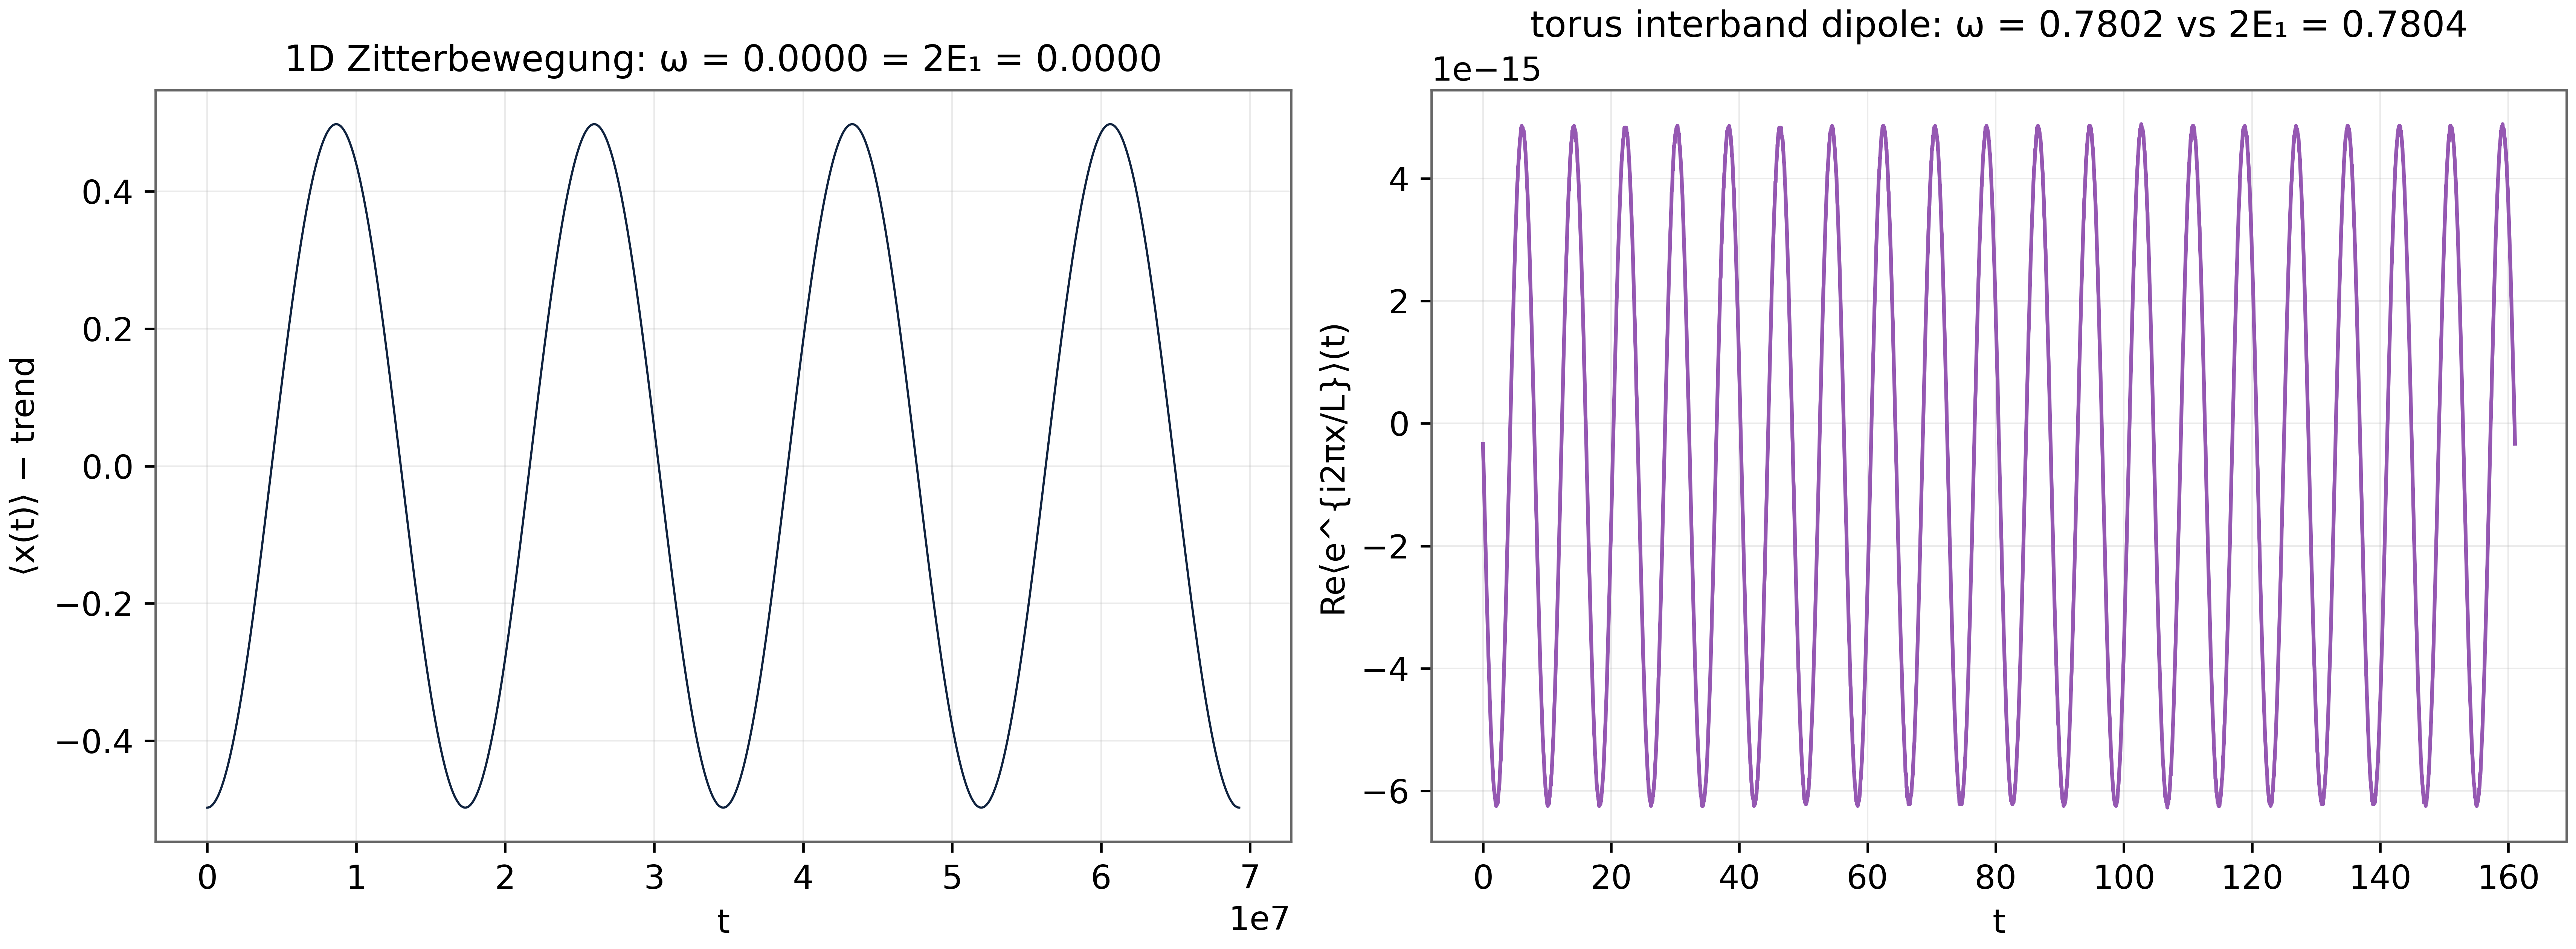
\includegraphics[max width=\columnwidth, max height=0.42\textheight]{figures/fig_D6_zitterbewegung.png}
\caption{Canonical D6 figure (600 dpi): dipole traces and their spectra for both instruments, produced by the original harness.}\label{fig:d6_1}
\end{figure}
\begin{figure}[htbp]\centering
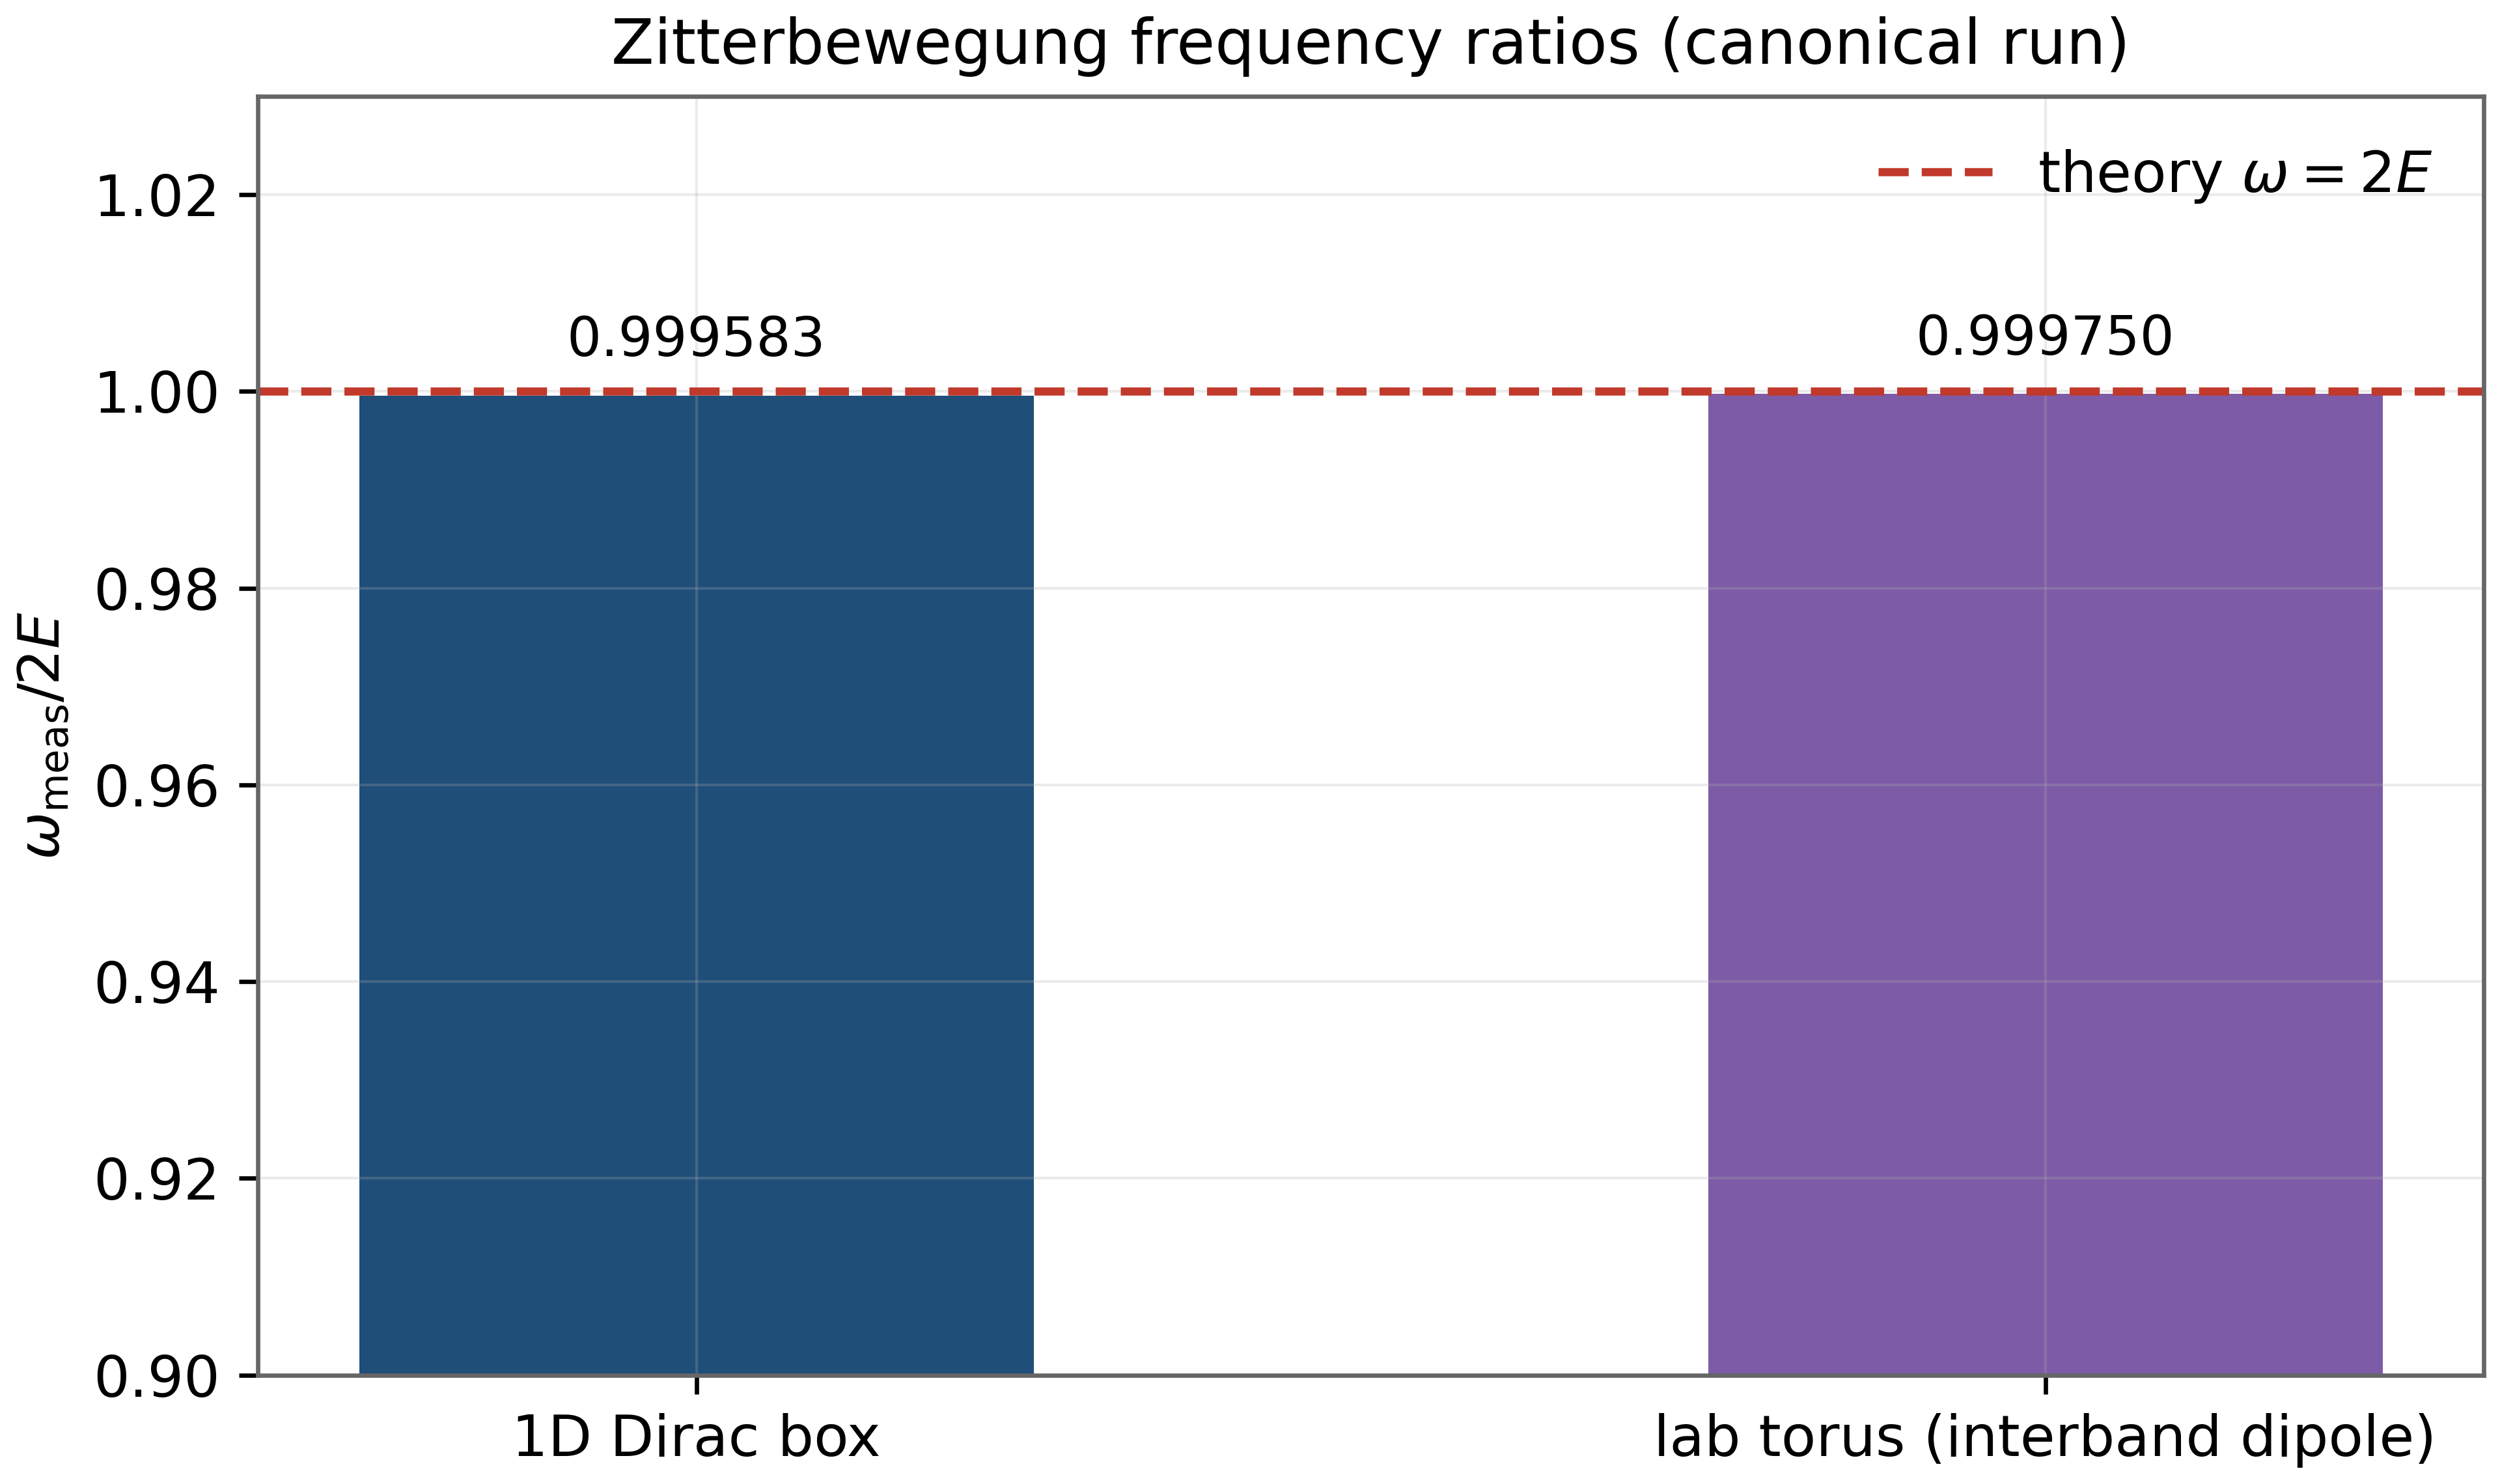
\includegraphics[max width=\columnwidth, max height=0.42\textheight]{figures/d06_extra_ratio_bars.png}
\caption{Companion bar panel built from the canonical CSV: measured $\omega/2E$ ratios against the theory line $1.0$.}\label{fig:d6_2}
\end{figure}

\section{Discussion}
Zitterbewegung completes the clean-suite identity proof, and its control design carries the laboratory's methodological signature: measure the effect, then kill it and measure again. The same pattern reappears in D9 (wall mode vs wall-less control), D10 (ζ cloud vs uniform and Poisson clouds) and D13 (orbit-driven vs generator-driven walls), which is why the clean suite should be read as much for its experimental grammar as for its numbers.

A natural extension is a driven Zitterbewegung spectroscopy: sweep the initial level and map the line $\omega = 2E$ across the whole clean spectrum, then repeat on the decorated operator to see whether the $\zeta$ phases perturb the beat. The box instrument makes this a small computation; the interpretation would feed directly into the D13 drive narrative.

\section{Reproducibility}
\begin{itemize}[leftmargin=1.2em, itemsep=0.15em]
\item \textbf{Single test:} \texttt{python3} \path{code/dirac_lab.py} \texttt{--test D6} (add \texttt{--quick} for a reduced pass; \texttt{--no-figures} to skip the 600-dpi figure).
\item \textbf{Canonical run:} \texttt{make all} regenerates the whole D1--D14 ledger into \path{results/}; this monograph's ledger is the verbatim per-check table of that run.
\item \textbf{Determinism:} seed 96 (parent convention); the $\zeta$ tables are the Odlyzko-derived files in \path{data/} with provenance in their headers.
\item \textbf{Figures:} the canonical figure was regenerated into this folder by the v1.4 harness (the original test function itself); companion panels are recomputed with the same modules (\path{scripts/make_extra_figures.py}). All figures are 600 dpi.
\item \textbf{Cross-verification:} Python-verified; the Julia cross-coverage map is \path{results/CROSS_VERIFICATION.md}.
\item \textbf{Artifacts in this folder:} \path{monograph.tex} (this document's source), \path{results.json} (machine-readable ledger), \path{figures/} (600-dpi figures), and the canonical CSV of the test.
\end{itemize}

\section*{References}
\begin{thebibliography}{99}\small
\bibitem{schrodinger} E. Schr"odinger, "Uber die kr"aftfreie Bewegung in der relativistischen Quantenmechanik, Sitzungsber. Preuss. Akad. Wiss. Phys.-Math. Kl. 24, 418 (1930).
\bibitem{dirac} P. A. M. Dirac, The quantum theory of the electron, Proc. R. Soc. A 117, 610 (1928).
\end{thebibliography}

\vfill
\noindent\rule{\textwidth}{0.4pt}\\[0.2em]
{\footnotesize\color{labgray} AB-Cloud Dirac Laboratory · per-test monograph series v1.4 · compiled with Tectonic (LaTeX) · all numbers traceable to \texttt{results/run\_20261006\_full\_v13} · \texttt{D6} of 14.}

\end{document}